\documentclass[american,aps,pra,reprint,floatfix,nofootinbib,superscriptaddress]{revtex4-2}
% General document formatting
\usepackage{tikz}
\usepackage[margin=0.7in]{geometry}
\usepackage{xintfrac}
% Documentation:
% https://ftp.cc.uoc.gr/mirrors/CTAN/macros/latex/contrib/parskip/parskip.pdf
\usepackage[utf8]{inputenc}

% Math packages:
\usepackage{amsmath,amssymb,amsfonts,amsthm}

% Our definitions:
\DeclareMathOperator{\smoothen}{smoothen}
\DeclareMathOperator{\mean}{mean}
\newcommand{\abs}[1]{\left|#1\right|}
\newcommand{\absmt}{\abs{m_{T}'}}

\usepackage{xcolor}
\newcommand{\bbk}[1]{\textcolor{green}{[VK: #1]}}
\newcommand{\DL}[1]{\textcolor{blue}{[DL: #1]}}
\newcommand{\NE}[1]{\textcolor{magenta}{[NE: #1]}}

\begin{document}

\title{Machine learning Fisher Information Metric from bitstrings}
\author{First Last}
\email{email}
\affiliation{USC affiliation}

\date{\today}

\begin{abstract}
We present a machine-learning based method ``Bitstring-ChiFc'' which,
given a dataset corresponding to a family of distributions of bitstrings
parameterized by a manifold, can produce a rough approximation
for the corresponding Fisher Information Metric.
We observe that for multiple toy models there are often enough simple patterns
in the data that this approach
achieves satisfactory approximation even for dataset sizes small
compared to the number of possible bitstrings.
\end{abstract}

\maketitle

\section{Presentation}
\subsection{Introduction}
Let's talk about phase transitions.  Consider the Hamiltonian
on a $2 \times L$ lattice given by the following equations.
\begin{equation}
  \label{eq:Hladder.1}
  H(s,K,U) = (1-s) H_0 + s H_1,
\end{equation}
\begin{equation}
  \label{eq:Hladder.2}
  H_0 = -\sum_{i=0}^{L-1} (X_{T_i} + X_{B_i}),
\end{equation}
\begin{multline}
  \label{eq:Hladder.3}
  H_1 = \sum_{i=0}^{L-1} \biggl(K Z_{T_i} Z_{T_{i+1}} - K Z_{T_i} Z_{B_i}
    - K Z_{B_i} Z_{B_{i+1}} \\
  - K Z_{T_i} + \frac{U}{2} Z_{B_i}\biggr).
\end{multline}
Here qubits $T_L$ and $B_L$ are identified with $T_0$ and $B_0$ respectively.

It is called ``Frustrated Ladder Hamiltonian'' and is schematically represented
by the following diagram:
\begin{center}
  \pgfmathparse{\columnwidth/10.7cm}%
  \edef\tikzscale{\pgfmathresult}%
  \begin{tikzpicture}[scale=\tikzscale]
    \foreach \x in {0,...,9}{
      \draw (\x,0) circle (0.3) node (n0x\x){$T_{\x}$};
      \draw (\x,-1) circle (0.3) node (n1x\x){$B_{\x}$};
      \draw (n0x\x) -- (n1x\x);
    }
    \foreach \x[count=\xnext from 1] in {0,...,8}{
      \draw[dotted,line width=1pt] (n0x\x) -- (n0x\xnext);
      \draw (n1x\x) -- (n1x\xnext);
    }
    \draw[dotted,line width=1pt] (-0.7,0) -- (n0x0);
    \draw (-0.7,-1) -- (n1x0);
    \draw[dotted,line width=1pt] (9.7,0) -- (n0x9);
    \draw (9.7,-1) -- (n1x9);
  \end{tikzpicture}
\end{center}
On this diagram of $L=10$ Frustrated Ladder Hamiltonian
the solid lines represent ferromagnetic couplings and
dotted lines --- antiferromagnetic couplings. For a fixed $L$
the Frustrated Ladder Hamiltonian depends on 3 parameters, $s, K, U$.
We set $K=1$ and consider the values $s\in[0,1]$, $U\in[0,1]$.

How would you find phase transitions of that Hamiltonian? For that particular
Hamiltonian people already know a couple of order parameters given by the
following equations.
\begin{equation}
  \label{eq:mt}
  \absmt = \abs{\sum_i Z_{T_i}(-1)^i}
\end{equation}
\begin{equation}
  \label{eq:mb}
  m_B = \sum_i Z_{B_i}
\end{equation}

These are called ``staggered magnetization of the top row'' and ``magnetization
of the bottom row'' respectively. For $L=10$ we can compute these for various
values of the parameters of the Hamiltonian and produce the following diagrams:
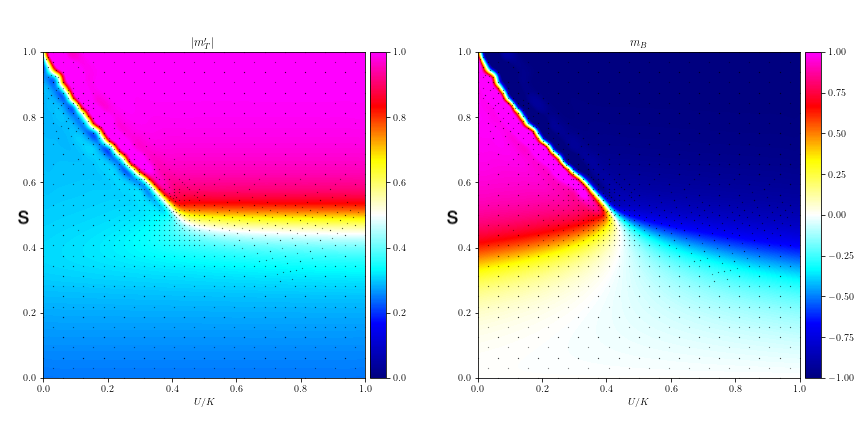
\includegraphics[width=\columnwidth]{lanczos_chi0_gp.png}

\section{TODO}
\begin{enumerate}
\item Complete presentation section above.
\item Write down the proofs for the fidelity susceptibility claims below.
\item Describe the models and practical results for them.
\end{enumerate}

\section{Introduction}
TODO:

Such a family can arise, e.g., from measurements of a low-temperature
Gibbs ensemble of Hamiltonians parametrized by a parameter $\lambda$.

\section{Classical Fidelity Susceptibility}
Classical fidelity between 2 probability distributions $p$ and $q$ of
bitstrings $z$ is defined as
\begin{equation}
  F_c(p, q) = \sum_{z} \sqrt{p(z) q(z)}.
\end{equation}
We are interested in the fidelity between bitstring distributions at different
$s$ (e.g. $s=s_1$ and $s=s_2$), which we will denote as $F_c(s_1, s_2)$.

\NE{This is an example of a commonly used in-line comment which is separated by color. I could say something like: "This sentence is awkward" or "Needs citation" or very meta "Please use enquote for real quotes and not literal quotes."}

Fidelity susceptibility is defined as the term $\chi_{F_c}(s)$ in the Taylor
expansion
\begin{equation}
\label{eq:Fcs.Tailor}
  F_c(s, s+\delta s) = 1 - \frac{\delta s^2}{2} \chi_{F_c}(s) + O(\delta s^3).
\end{equation}
For such Taylor expansion to exist it is sufficient that the probabilities have
a Taylor expansion up to $O(\delta s^3)$. More generally, probability
distribution can depend on a point $\lambda$ on a manifold $\Lambda$,
in which case the Tailor expansion \eqref{eq:Fcs.Tailor} would become
\begin{equation}
\label{eq:Fcl.Tailor}
  F_c(\lambda, \lambda+\delta \lambda) = 1 - \frac{\delta \lambda_{j} \delta \lambda_k}{2} \chi_{F_c}^{jk}(\lambda) + O(\delta \lambda^3).
\end{equation}

\subsection{Classical and quantum fidelity susceptibility}
Fact 1: For pure states $\mathbb{E}\chi_{F_c} (s) = \frac12 \chi_F (s)$
where the expectation is over all orthogonal bases to perform the measurement in.

TODO:proof

Fact 2: For computational basis measurement of a non-degenerate ground state
of a real-valued Hamiltonian $H$, then $\chi_{F_c}(s) = \chi_F(s)$
almost everywhere.

TODO:proof

\section{Problem setup}
\begin{itemize}
  \item In this work we consider a family of distributions of
bitstrings $\{\mathcal{D}_{\lambda}\}_{\lambda \in \Lambda}$, each of length $n$.
  \item We are given a finite sample $\mathcal{D}_{\textrm{train}}$ of size $N$
  of pairs $(\lambda, z)$ s.t. $P(z|\lambda) = P_{\mathcal{D}_{\lambda}}(z)$.
  \item We are also given (possibly implicitly via coordinate description of $\Lambda$) a naive metric $g^0$ on $\Lambda$.
  \item We are asked to estimate the Fisher information metric $g$ on $\Lambda$ corresponding to distributions $\mathcal{D}_{\lambda}$.
  \item Locations with high $g / g^0$ are then considered to be conjectured locations of possible phase transitions.
\end{itemize}

We focus on the task of identifying phase transitions in that
family. Rigorously speaking, phase transitions are only defined
in the limit $n\to\infty$, while we are dealing with finite size systems.
A solution to that is to look at Fisher information metric: high distances according to Fisher information metric for points close according to naive metric likely correspond to phase transitions.

\section{Bitstring-ChiFc method}
In this work we propose the following method:
\begin{itemize}
  \item Collect training dataset $\mathcal{D}_{\chi_{F_c}\textrm{-train}}$ of
  the form $(\lambda_0, \delta \lambda, z, y)$, where $z$ is sampled from
  $p(\bullet, \lambda=\lambda_{z})$,
  $p_{+} = p(\lambda_{z} = \lambda_0 + \delta \lambda / 2| \lambda_{z} = \lambda_0 \pm \delta \lambda / 2)$, and
    $\mathbb{E}(y|\lambda_0, \delta \lambda, z) = p_{+}$.
    In practice $y \in \{0, 1\}$.
    Do it in the following way:
    \begin{itemize}
      \item Consider $\mathcal{D}_{\textrm{train}}$ consisting of pairs
      $(z, \lambda)$.
      \item Sample pairs $(z_{i{+}}, \lambda_{i{+}})$,
      $(z_{i{-}}, \lambda_{i{-}})$ from $\mathcal{D}_{\textrm{train}}$.
      \item Compute $\lambda_i = (\lambda_{i{+}} + \lambda_{i{-}})/2$,
      $\delta \lambda_i = \lambda_{i{+}} - \lambda_{i{-}}$.
      \item Add tuples $(\lambda_i, \delta \lambda_i, z_{i{+}}, 1)$ and $(\lambda_i, \delta \lambda_i, z_{i{-}}, 0)$ to the dataset $\mathcal{D}_{\chi_{F_c}\textrm{-train}}$.
    \end{itemize}
  \item Train a model $M$, which given $(\lambda_0, \delta \lambda, z)$
  will predict $l = M(\lambda_0, \delta \lambda, z)$
  s.t. $p_{+} = (1+e^{-l \cdot \delta \lambda})^{-1}$.
  Do this by minimizing cross-entropy loss on the dataset
  $\mathcal{D}_{\chi_{F_c}\textrm{-train}}$.
  \item Estimate
  \begin{equation}
  \chi_{F_c}^{jk}(\lambda) = \smoothen\left(\lambda_1 \mapsto
  \mean_{(z, \lambda_1) \in \mathcal{D}_{\textrm{train}}}
  M(\lambda_1, 0, z)^{j}M(\lambda_1, 0, z)^{k}\right)(\lambda).
  \end{equation}
\end{itemize}

TODO: expand the explanation.

    \begin{multline*}
      \chi_{F_c}(\lambda) = \lim_{\delta \lambda\to 0} \frac2{\delta \lambda^2} \left(1 - \mathbb{E}_{z\sim Q(\bullet)} \frac{\sqrt{P(z|\lambda-\delta \lambda/2)P(z|\lambda+\delta \lambda/2)}}{Q(z)}\right)
      \\ \simeq \lim_{\delta \lambda\to 0} \mathbb{E}_{Q}\frac2{\delta \lambda^2}\frac{2\sinh^2(l\delta \lambda/4)}{\cosh(l\delta \lambda/2)} \simeq \frac14 \mathbb{E}_{z|\lambda} M(\lambda, 0, z)^2.
    \end{multline*}

TODO: models

TODO: experiments

\end{document}
